

%----------------------------------------------------------------------------------------
%	PACKAGES AND OTHER DOCUMENT CONFIGURATIONS
%----------------------------------------------------------------------------------------

\documentclass[12pt]{article}
 
\usepackage{polski}
\usepackage[polish]{babel}
\usepackage[utf8]{inputenc}
\usepackage{datetime}
\usepackage{graphicx} 
\usepackage{tikz} 
\usepackage{amsmath}
\usepackage{epstopdf}
\usepackage{array,booktabs}
\usepackage{float}
%\usepackage[colorlinks=true]{hyperref}
%\usepackage[all]{hypcap}
%\usepackage{showframe}
\usepackage{geometry}
 \geometry{
 a4paper, 
 left=30mm,
 right=30mm,
 top=30mm,
 bottom=30mm,
 }
 
\usepackage{listings}
\usepackage{color}

\definecolor{mygreen}{rgb}{0,0.6,0}
\definecolor{mygray}{rgb}{0.5,0.5,0.5}
\definecolor{mymauve}{rgb}{0.58,0,0.82}

\lstset{ %
  backgroundcolor=\color{white},   % choose the background color; you must add \usepackage{color} or \usepackage{xcolor}
  basicstyle=\footnotesize,        % the size of the fonts that are used for the code
  breakatwhitespace=false,         % sets if automatic breaks should only happen at whitespace
  breaklines=true,                 % sets automatic line breaking
  captionpos=b,                    % sets the caption-position to bottom
  commentstyle=\color{mygreen},    % comment style
  deletekeywords={...},            % if you want to delete keywords from the given language
  escapeinside={\%*}{*)},          % if you want to add LaTeX within your code
  extendedchars=true,              % lets you use non-ASCII characters; for 8-bits encodings only, does not work with UTF-8
  frame=single,                    % adds a frame around the code
  keepspaces=true,                 % keeps spaces in text, useful for keeping indentation of code (possibly needs columns=flexible)
  keywordstyle=\color{blue},       % keyword style
  language=Octave,                 % the language of the code
  morekeywords={*,...},            % if you want to add more keywords to the set
  numbers=left,                    % where to put the line-numbers; possible values are (none, left, right)
  numbersep=5pt,                   % how far the line-numbers are from the code
  numberstyle=\tiny\color{mygray}, % the style that is used for the line-numbers
  rulecolor=\color{black},         % if not set, the frame-color may be changed on line-breaks within not-black text (e.g. comments (green here))
  showspaces=false,                % show spaces everywhere adding particular underscores; it overrides 'showstringspaces'
  showstringspaces=false,          % underline spaces within strings only
  showtabs=false,                  % show tabs within strings adding particular underscores
  stepnumber=1,                    % the step between two line-numbers. If it's 1, each line will be numbered
  stringstyle=\color{mymauve},     % string literal style
  tabsize=2,                       % sets default tabsize to 2 spaces
  title=\lstname                   % show the filename of files included with \lstinputlisting; also try caption instead of title
}
 
\newdate{create_date}{26}{05}{2014}

%----------------------------------------------------------------------------------------

%----------------------------------------------------------------------------------------
% TIKZ PACKAGES
%----------------------------------------------------------------------------------------

\usetikzlibrary{arrows, calc}

%----------------------------------------------------------------------------------------

\begin{document}

\begin{titlepage}

\newcommand{\HRule}{\rule{\linewidth}{0.5mm}}
% Defines a new command for the horizontal lines, change thickness here

\center
% Center everything on the page
 
%----------------------------------------------------------------------------------------
%	LOGO SECTION
%----------------------------------------------------------------------------------------


\includegraphics[width=6cm]{../res/img/logo.png}\\[1cm]
% Include a department/university logo - this will require the graphicx package
 
%----------------------------------------------------------------------------------------
 
%----------------------------------------------------------------------------------------
%	HEADING SECTIONS
%----------------------------------------------------------------------------------------

\textsc{\LARGE Akademia Górniczo-Hutnicza \\[0.2cm]
im. Stanisława Staszica w Krakowie}\\[1.5cm]
% Name of your university/college

\textsc{\Large Podstawy Automatyki}\\[0.5cm]
% Major heading such as course name

%----------------------------------------------------------------------------------------
%	TITLE SECTION
%----------------------------------------------------------------------------------------

\HRule \\[0.5cm]
{ \huge \bfseries Dyskretne układy regulacji \\[0.3cm] oraz \\[0.5cm] Analiza
serwomechanizmu \\[0.2cm] przekaźnikowego z wykorzystaniem płaszczyzny
fazowej}\\[0.3cm]
% Title of your document
\HRule \\[1.5cm]
 
%----------------------------------------------------------------------------------------
%	AUTHOR SECTION
%----------------------------------------------------------------------------------------

% \begin{minipage}{0.4\textwidth}
% \begin{flushleft} \large
% \emph{Author:}\\
% Konrad \textsc{Adasiewcz} % Your name
% \end{flushleft}
% \end{minipage}
% ~
% \begin{minipage}{0.4\textwidth}
% \begin{flushright} \large
% \emph{Supervisor:} \\
% dr inż. Paweł \textsc{Rotter} % Supervisor's Name
% \end{flushright}
% \end{minipage}\\[4cm]

% If you don't want a supervisor, uncomment the two lines below and remove the section above
\flushright
\Large \emph{Autorzy:}\\
Konrad \textsc{Adasiewcz}\\[0.1cm] % Your name
Michał \textsc{Maciejewski}\\[3cm] % Your name

%----------------------------------------------------------------------------------------
%	DATE SECTION
%----------------------------------------------------------------------------------------
Data wykonania ćwiczenia: \\
{\large \displaydate{exercise_date}}\\[1cm]


\vfill % Fill the rest of the page with whitespace

\end{titlepage}

\section{Wstęp}

\subsection{Cel ćwiczenia}

Celem ćwiczenia jest przeprowadzenie linearyzacji modelu matematycznego
podgrzewanego zbiornika z cieczą, dla wybranego punktu pracy obiektu.


\begin{figure}[!htb]
	\begin{center}
		\includegraphics[page=2,width=14cm,trim=3cm 3cm 3cm 17.5cm,clip]
		{../res/img/schemat.pdf}
	\end{center}
	\caption{Schemat modelowanego zbiornika}
\end{figure}

Ogólnie rzecz biorąc linearyzacja polega na rozwinięciu w szereg Taylora rzędu
pierwszego funkcji opisującej układ równań różniczkowych dla punktu pracy
będącego stanem ustalonym obiektu. Wtedy mamy:

\begin{equation}
	f(x,u)\approx A\cdot(x-x_0)+B\cdot(u-u_0)
\end{equation}

gdzie:

\begin{equation*}
	A=\frac{\partial f}{\partial x}(x_0,u_0)
\end{equation*}

\begin{equation*}
	B=\frac{\partial f}{\partial u}(x_0,u_0)
\end{equation*}

A to jest równanie stanu układu liniowego w notacji macierzowej, jednak dla
zmiennych odchyłkowych, o czym należy pamiętać.

\newpage

\section{Model nieliniowy}

Modelowany zbiornik opisuje następujące równanie (układ równań):

\begin{equation}
	\begin{cases}
		\dot{V} = \dfrac{1}{\rho}(w_i-w) \\[0.3cm]
		\dot{T} = \dfrac{w_i(T_i-T)}{\rho V} + \dfrac{Q}{C\rho V} \\
	\end{cases}
	\label{equ:rstanun}
\end{equation}

gdzie:

\begin{equation*}
	\begin{cases}
		\rho = 1000 [\frac{kg}{m^3}] \\[0.3cm]
		C = 1820 [\frac{J}{kg\cdot K}] \\
	\end{cases}
\end{equation*}

Co wprowadziłem do \textsc{Matlab}'a w następującej postaci:


\begin{lstlisting}[language=matlab]
function [xp] = rown_stanu(t,x,u)

%x=[V T]
%u=[wi w Ti Q] 

C=1820;
ro=1000;

xp(1,1)=(u(2)-u(1))/ro;
xp(2,1)=u(1)*(u(3)-x(2))/(ro*x(1))+u(4)/(ro*x(1)*C);

end
\end{lstlisting}

Przy pomocy metod numerycznych jesteśmy w stanie uzyskać rozwiązanie
równania różniczkowego dla zadanych warunków początkowych. Przy pomocy solvera
\textit{ode45} zawartego w pakiecie \textsc{Matlab}, wyznaczyłem odpowiedź
systemu dla przykładowego sterowania i warunków początkowych, tj.:

\begin{equation*}
	\begin{cases}
		w_i = w = 0.4 [\frac{kg}{s}]\\
		T_i = 293[K]\\
		Q=8000[W]\\[0.2cm]
		\begin{cases}
			V_0=0.04[m^3]\\
			T_0=293[K]
		\end{cases}
	\end{cases}
\end{equation*}

\newpage

\begin{figure}[!htb]
	\begin{center}
		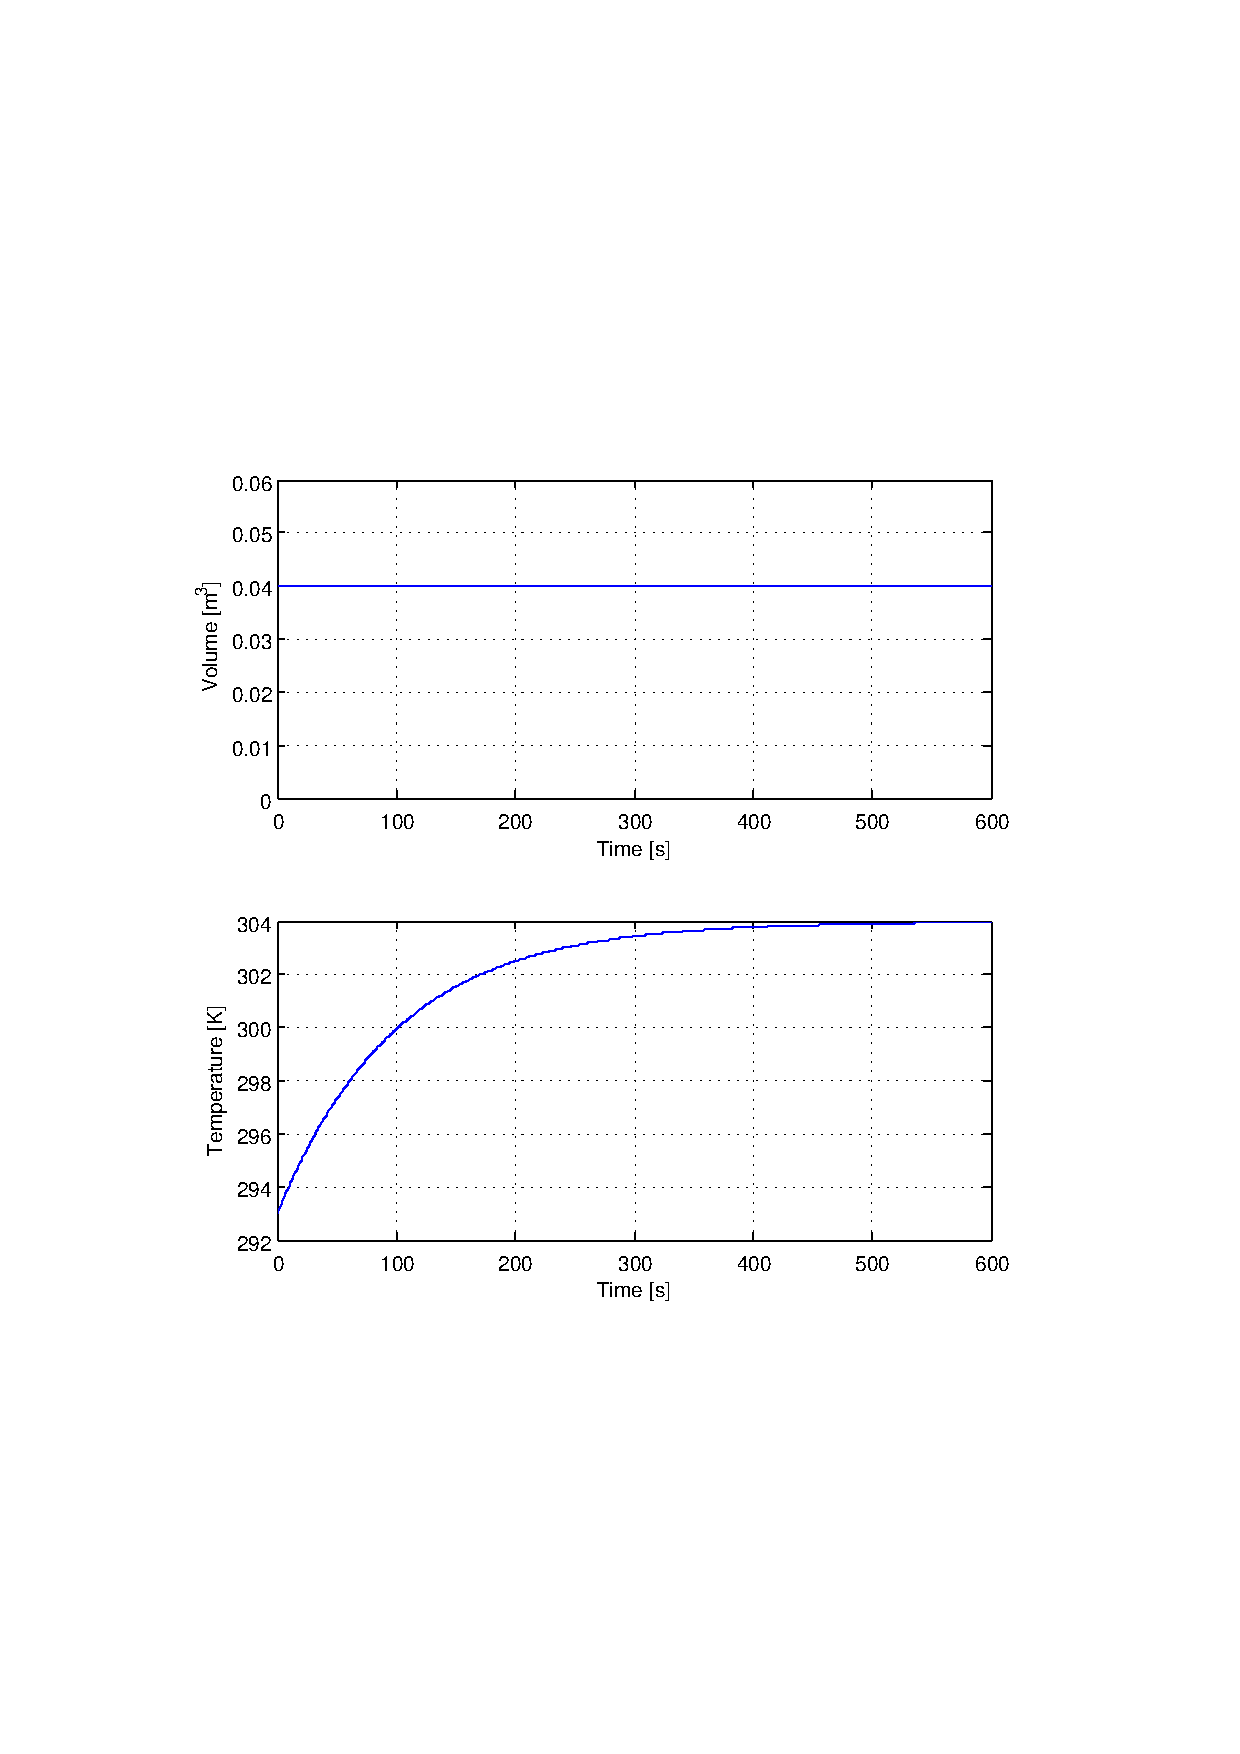
\includegraphics[width=14cm,trim=3cm 7cm 3cm 8cm,clip]
		{../res/img/nonl_u0_x0.pdf}
	\end{center}
	\caption{Odpowiedź systemu na przykładowy zestaw parametrów}
\end{figure}

\newpage

\section{Model zlinearyzowany}

Chcąc zlinearyzować system dynamiczny wykorzystując pakiet \textsc{Matlab}
potrzebny jest jego model w \textsc{Simulink}'u. W celu jego wykonania
potrzebujemy tzw. S-Funkcję, która wykorzystywać będzie wcześniej napisane
równanie stanu. Mając to jesteśmy już w stanie zbudować model.

\begin{lstlisting}[language=matlab]
function [sys,x0,str,ts]=zbiornik_sfcn(t,x,u,flag,V0,T0) 

switch flag 
     case 0
          str = []; 
          ts = [0 0]; 
          s = simsizes; 
               s.NumContStates = 2;
               s.NumDiscStates = 0;
               s.NumOutputs = 2;
               s.NumInputs = 4;
               s.DirFeedthrough = 0;
               s.NumSampleTimes = 1;
          sys = simsizes(s); 
          x0 = [V0, T0]; 
     case 1
          sys = rown_stanu(t,x,u); 
     case 3
          sys = x; 
     case {2 4 9} 
          sys =[]; 
     otherwise 
          error([ 'unhandled flag =',num2str(flag)]); 
end 
\end{lstlisting}

Chcąc zlinearyzować model należy przyjąć punkt pracy w okolicy którego
linearyzujemy system. Przyjmuję punkt:

\begin{equation*}
	\tilde{x} =
	\begin{bmatrix}
		\tilde{V} \\
		\tilde{T}
	\end{bmatrix} =
	\begin{bmatrix}
		0.04 \\
		303
	\end{bmatrix}
\end{equation*}

Mając przyjęty punkt pracy należy wyznaczyć sterowanie, dla którego zostaje on
osiągnięty jako stan ustalony.

\newpage

\subsection{Sterowanie wyznaczone numerycznie}

Sterowanie punktu pracy można wyznaczyć numerycznie. Po wykonaniu modelu należy
wykorzystać funkcję \textit{trim}, która przyjmuje jako argumenty nazwę pliku
pod którą zapisaliśmy model, wektory sterowania, stanu, wyjścia oraz macierze,
które wyznaczają parametry które chcemy aby pozostały stałe.

Przy wykorzystaniu funkcji \textit{trim} i daniu jej większej swobody w szukaniu
stanu ustalonego (parametr $w_i$ może się zmieniać) otrzymujemy wektor sterowania:

\begin{equation*}
	\tilde{u} =
	\begin{bmatrix}
		\tilde{w_i} \\
		\tilde{w} \\
		\tilde{T_i} \\
		\tilde{Q}
	\end{bmatrix} =
	\begin{bmatrix}
		0.4396 \\
		0.4396 \\
		293 \\
		8000
	\end{bmatrix}
\end{equation*}

\subsection{Sterowanie wyznaczone analitycznie}

Sterowanie można również wyznaczyć analitycznie. W tym celu należy rozwiązać
układ równań:

\begin{equation*}
	\begin{cases}
		0 = \dfrac{1}{\rho}(w_i-w) \\[0.3cm]
		0 = \dfrac{w_i(T_i-303)}{\rho 0.04} + \dfrac{Q}{C\rho 0.04} \\
	\end{cases}
\end{equation*}

Ponieważ mamy 2 równania a aż 4 zmienne, należy kilka zmiennych ograniczyć
pewnymi warunkami, lub narzucić ich wartość. $w_i$ oraz $T_i$ są parametrami
dostarczanej cieczy i zakładam, że nie można ich zmienić. Z uwagi na pierwsze
równanie powyższego układu równań wynika iż $w=w_i$ więc tym parametrem również nie można
manipulować. Zmieniamy więc jedynie $Q$ i układ równań sprowadza się do jednego
równania z którego bez problemu można wyliczyć $\tilde{Q}=7280[W]$.

Zatem sterowanie w ustalonym punkcie pracy wynosi:

\begin{equation*}
	\tilde{u} =
	\begin{bmatrix}
		\tilde{w_i} \\
		\tilde{w} \\
		\tilde{T_i} \\
		\tilde{Q}
	\end{bmatrix} =
	\begin{bmatrix}
		0.4 \\
		0.4 \\
		293 \\
		7280
	\end{bmatrix}
\end{equation*}

\newpage

\subsection{Porównanie}

W obu przypadkach przebiegi czasowe wyjść systemu zlinearyzowanego idealnie
pokrywają się z odpowiedziami właściwego modelu, nie ma sensu ich więc
przytaczać. Wobec tego poniżej zamieszczam przeieg różnicy temperatury dla
stanu początkowego:

\begin{equation*}
	\begin{cases}
		V_0=0.04[m^3]\\
		T_0=293[K]
	\end{cases}
\end{equation*}

i sterowań wyznaczonych w poprzednich podpunktach.

\begin{figure}[!htb]
	\begin{center}
		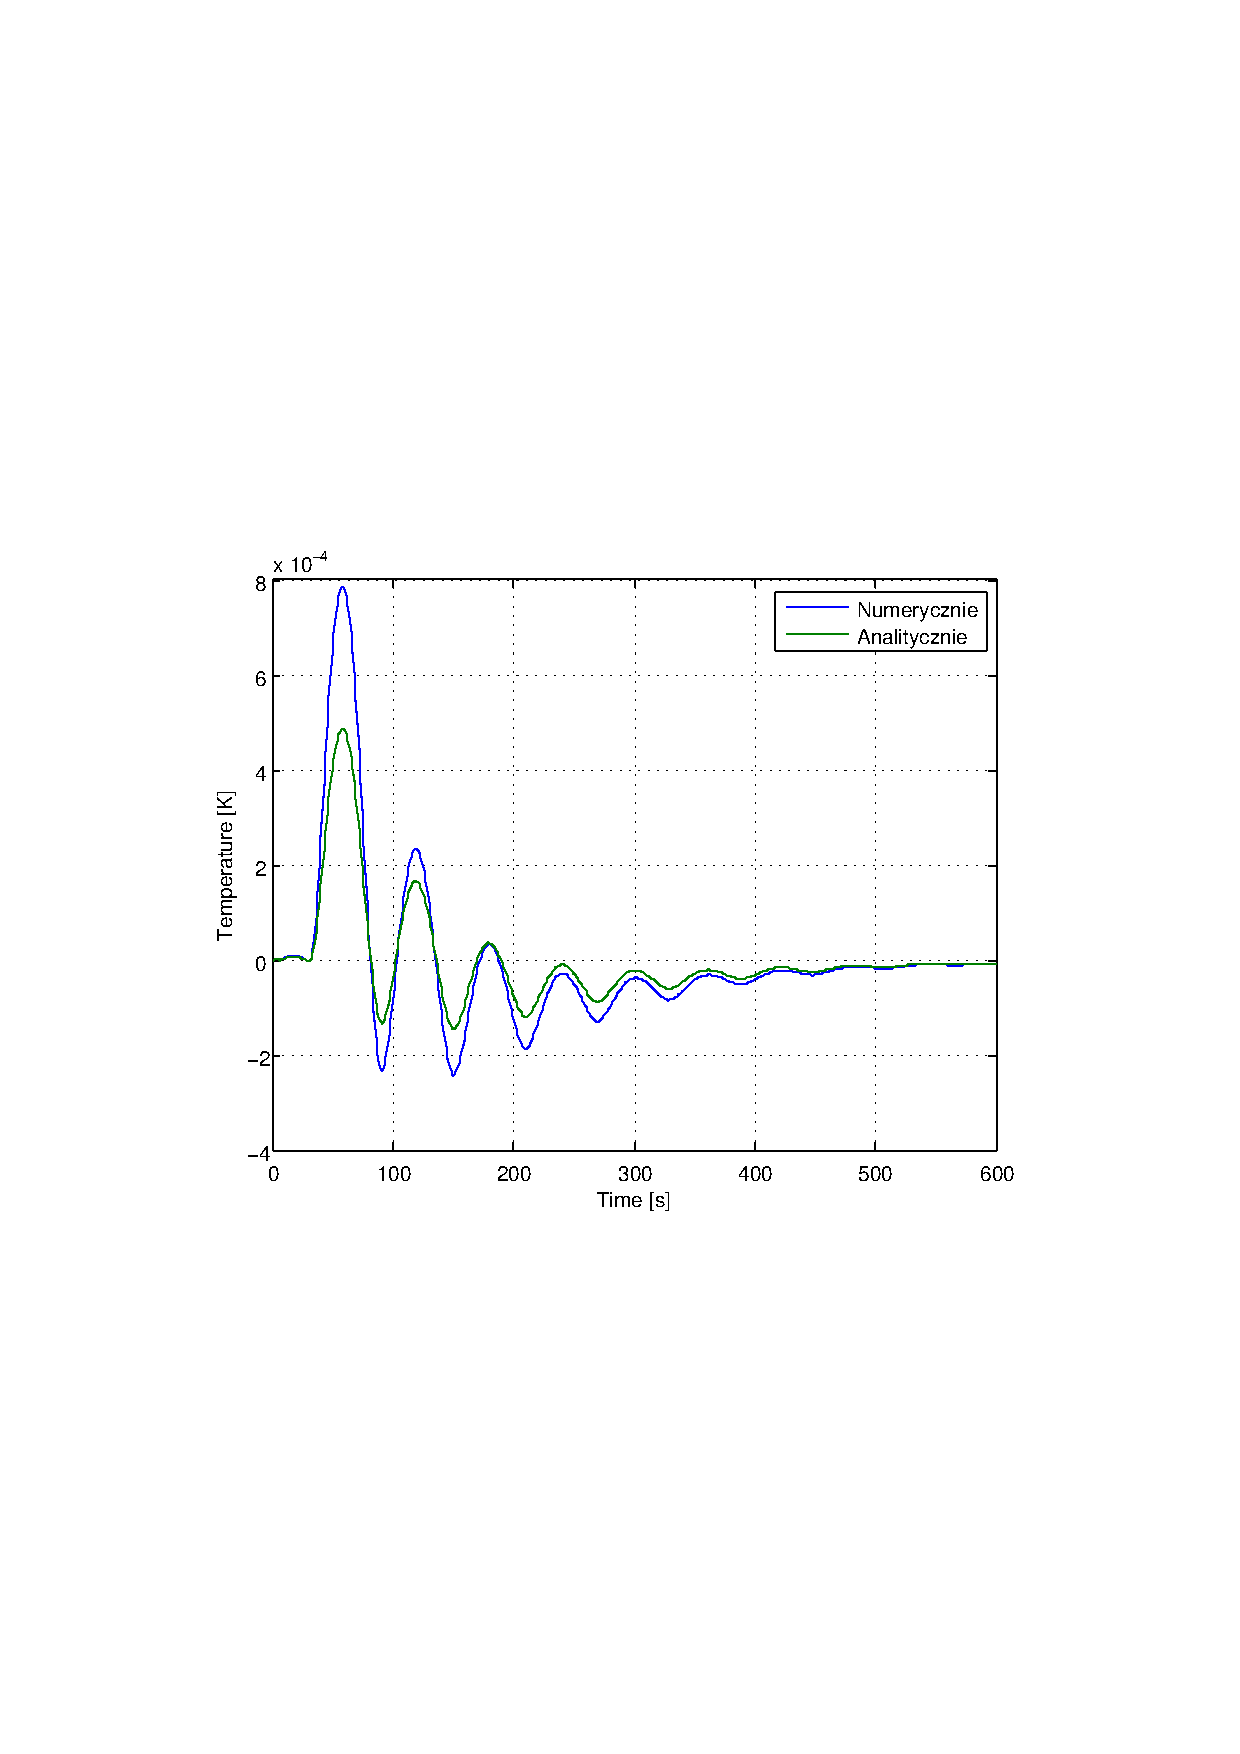
\includegraphics[width=12cm,trim=3cm 9cm 3cm 9cm,clip] 
		{../res/img/error12.pdf}
	\end{center}
	\caption{Przebiegi różnicy temperatury obu modeli}
\end{figure}

Przebiegi objętości w czasie są idealne z uwagi na równość $w_i=w$.

Jak widać obie aproksymacje oferują bardzo wysoki poziom dokładności.

\section{Wnioski}

Jak widać aproksymacja liniowa systemów nieliniowych jest w pobliżu punktu pracy
ich dobrym przybliżeniem, co może w niektórych przypadkach znacznie uprościć ich
analizę, szczególnie stabilnościową. Warto również zauważyć, iż wpływ
na dokładność zlinearyzowanego modelu ma wybór sterowania, który będzie
zapewniał to, iż wybrany punkt pracy będzie stanem ustalonym. Ma to
związek z kształtem funkcji opisującej nieliniowe równanie stanu. Im bardziej
przypomina ona linię prostą, (płaszczyznę, hiperpłaszczyznę) w otoczeniu punktu
pracy tym lepszą aproksymację uzyskamy.

\end{document}